\documentclass[fleqn]{beamer}
\usepackage[english]{babel}

\usepackage{amsmath,amssymb}
\usepackage{graphicx}

% vertical separator macro
\newcommand{\vsep}{
  \column{0.0\textwidth}
    \begin{tikzpicture}
      \draw[very thick,black!10] (0,0) -- (0,7.3);
    \end{tikzpicture}
}

% More space between lines in align
\setlength{\mathindent}{0pt}

% Beamer theme
\usetheme{UniVienna}
\usefonttheme[onlysmall]{structurebold}
\mode<presentation>
\setbeamercovered{transparent=10}

% align spacing
\setlength{\jot}{0pt}

\setbeamertemplate{navigation symbols}{}%remove navigation symbols

\title{Hiding Executable Code in Data Files}
\author{Samuel Šulovský}
\institute[University of Vienna]{Faculty of Computer Science, University of Vienna}
\date{\today}

\begin{document}
\begin{frame}
  \titlepage
\end{frame}

\begin{frame}
  \frametitle{Outline}
  \begin{columns}[T]
    \column{\textwidth}
    \begin{itemize}
      \item What Are Files?
      \item Lazarus APT BMP RAT Attack
      \item Malware Recreation
      \item Evaluation, Discussion, Conclusions
    \end{itemize}
  \end{columns}
\end{frame}

% ------ SEC: What are files?

\begin{frame}
  \frametitle{What Are Files?}
  \begin{columns}[T]
    \column{\textwidth}
    \begin{quote}
      A file is a named collection of related information that is recorded on secondary storage. From a user's perspective, 
      a file is the smallest allotment of logical secondary storage; that is, data cannot be written to secondary storage 
      unless they are within a file.
    \end{quote}
    Silberschatz et al. \emph{Operating System Concepts}
  \end{columns}
\end{frame}

\begin{frame}
  \frametitle{What Are Files?}
  \begin{columns}[T]
    \column{\textwidth}
    \begin{itemize}
      \item Files hold \emph{arbitrary} data -- binary, numeric, ASCII...
      \item Outward characteristics: file name and file \emph{extension}
      \item Interpretation of a file's contents is always "guesswork" 
    \end{itemize}
  \end{columns}
\end{frame}

\begin{frame}
  \frametitle{What Are Files?}
  \begin{columns}[T]
    \column{\textwidth}
    \begin{itemize}
      \item File extensions help us make a more accurate guess...
    \end{itemize}
    \begin{figure}[H]
      \centering
      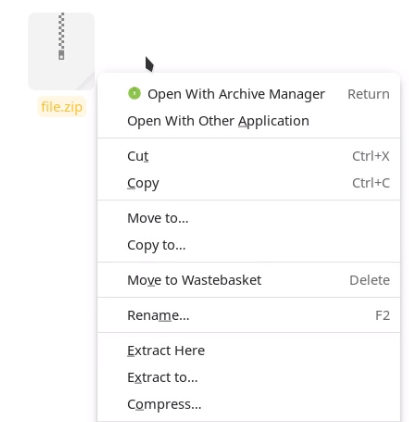
\includegraphics[scale=0.5]{images/is_it_an_archive.png}
    \end{figure}
  \end{columns}
\end{frame}

\begin{frame}
  \frametitle{What Are Files?}
  \begin{columns}[T]
    \column{\textwidth}
    \begin{itemize}
      \item But they are ultimately arbitrary!
    \end{itemize}
    \begin{figure}[H]
      \centering
      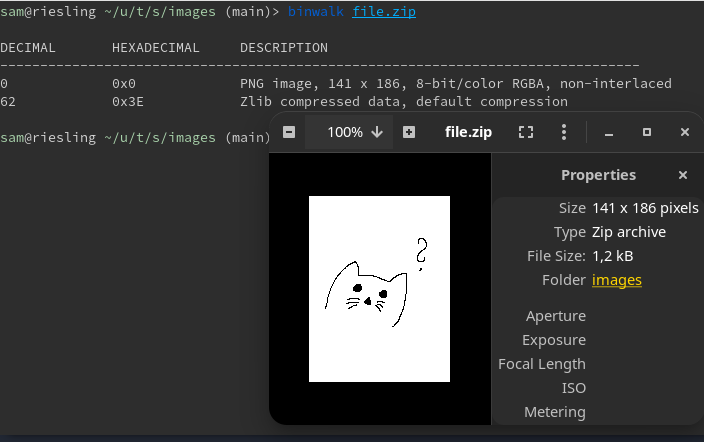
\includegraphics[scale=0.5]{images/lies_and_deciet_it_was_not_an_archive.png}
    \end{figure}
  \end{columns}
\end{frame}

\begin{frame}
  \frametitle{What Are Files?}
  \begin{columns}[T]
    \column{\textwidth}
    \begin{itemize}
      \item Trusting files to contain what they say they do can be a security risk
      \item Some file formats are more exploitable than others
      \item Studied example: the PNG file format
    \end{itemize}
  \end{columns}
\end{frame}

\begin{frame}
  \frametitle{What Are Files?}
  \begin{columns}[T]
    \column{\textwidth}
    \begin{quote}
    The first eight bytes of a PNG file always contain the following (decimal) values:
    \emph{137 80 78 71 13 10 26 10}

    This signature indicates that the remainder of the file contains a single PNG image, 
    consisting of a series of chunks beginning with an \emph{IHDR} chunk and ending 
    with an \emph{IEND} chunk.
    \end{quote}
    W3C \emph{PNG Specification}
  \end{columns}
\end{frame}

\begin{frame}
  \frametitle{What Are Files?}
  \begin{columns}[T]
    \column{0.5\textwidth}
    \begin{itemize}
      \item PNG data stream is terminated, all input after IEND is ignored
      \item Can we still append to the file? Sure!
    \end{itemize}
    \column{0.5\textwidth}
    \begin{figure}[H]
      \centering
      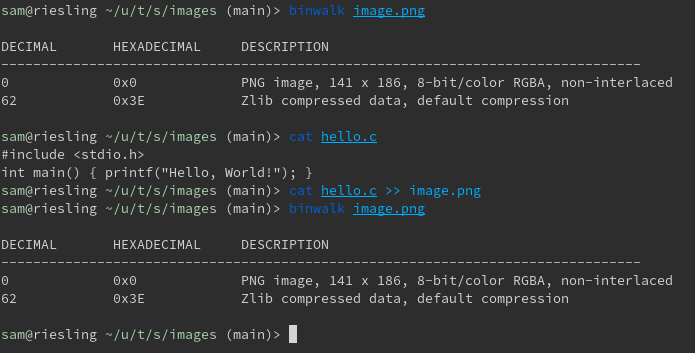
\includegraphics[scale=0.33]{images/hiding_data_after_iend.png}
    \end{figure}
  \end{columns}
\end{frame}

\begin{frame}
  \frametitle{What Are Files?}
  \begin{columns}[T]
    \column{\textwidth}
    \begin{itemize}
      \item Can we make the data less visible in the PNG data stream?
    \end{itemize}
    \begin{figure}[H]
      \centering
      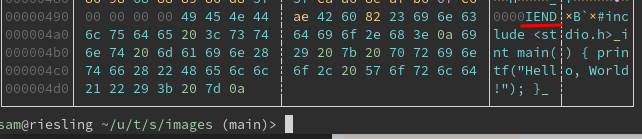
\includegraphics[scale=0.5]{images/hex_dump_after_iend.png}
    \end{figure}
  \end{columns}
\end{frame}

\begin{frame}
  \frametitle{What Are Files?}
  \begin{columns}[T]
    \column{\textwidth}
    \begin{itemize}
      \item Idea: masquerade as part of the PNG data stream!
      \item Compress the data using the same compression as the PNG uses
      \item Move the IEND terminator after our new data stream
    \end{itemize}
    \begin{figure}[H]
      \centering
      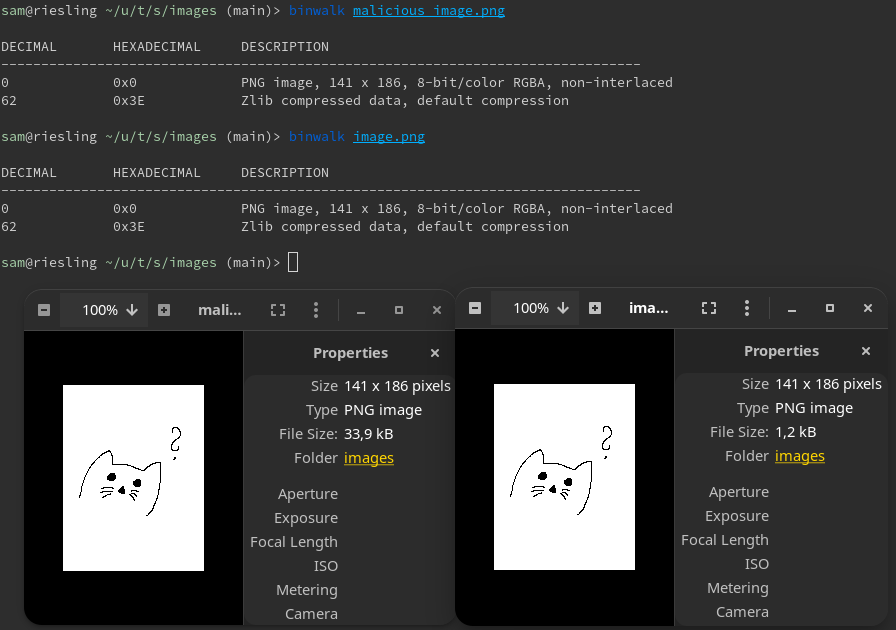
\includegraphics[scale=0.33]{images/hidden_perfectly.png}
    \end{figure}
  \end{columns}
\end{frame}

\begin{frame}
  \frametitle{What Are Files?}
  \begin{columns}[T]
    \column{\textwidth}
    \begin{itemize}
      \item Easier way to hide executable code in data files: document formats
      \item Micorsoft Office Suite has \emph{macro-enabled documents}
      \item Allows user to write code to be run from the document
      \item Very blatant security risk!
    \end{itemize}
    \begin{figure}[H]
      \centering
      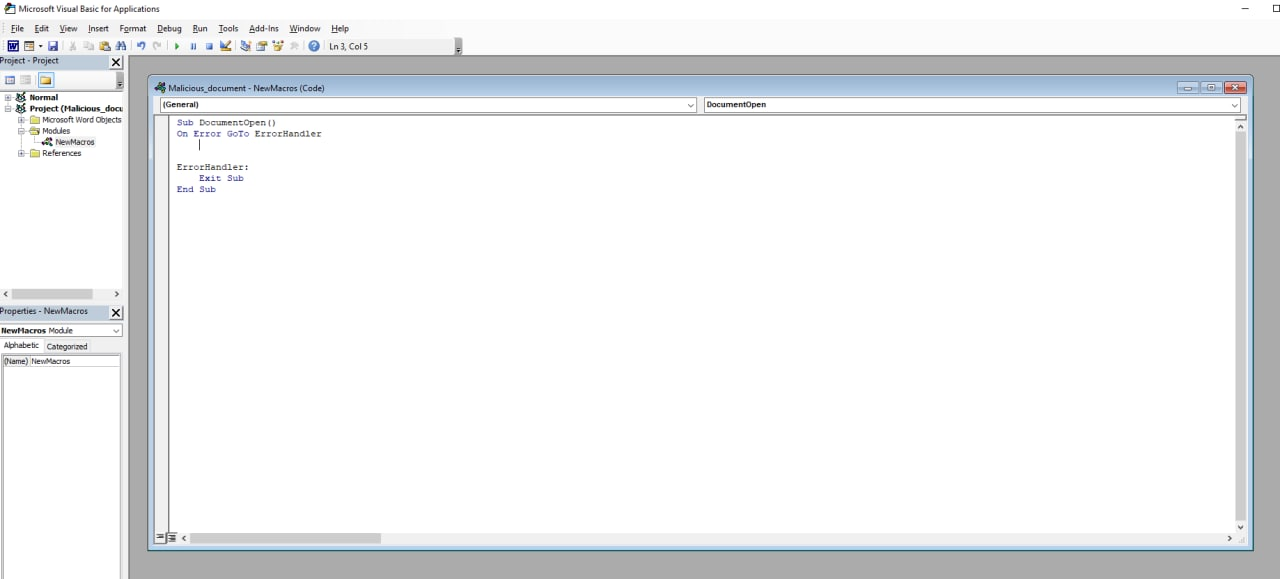
\includegraphics[scale=0.33]{images/ms_office_macro_editor.jpg}
    \end{figure}
  \end{columns}
\end{frame}

\begin{frame}
  \frametitle{What Are Files?}
  \begin{columns}[T]
    \column{\textwidth}
    \begin{itemize}
      \item Macros are disabled by default, with a pop-up option to enable them
      \item "A design comedy of errors with tragic security consequences" - Gutfleisch et al. 2021
      \item Remain a prominent attack vector, usually used to drop a payload
    \end{itemize}
    \begin{figure}[H]
      \centering
      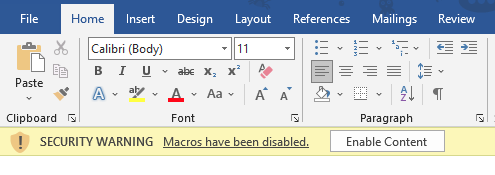
\includegraphics[scale=0.5]{images/macro_security_popup.png}
    \end{figure}
  \end{columns}
\end{frame}

% ------ Lazarus Slides
\begin{frame}
  \frametitle{Lazarus APT BMP RAT Attack}
  \begin{columns}[T]
    \column{\textwidth}
    \begin{itemize}
      \item We studied an attack thought to be perpetrated by Lazarus Group
      \item Thought to be a state-sponsored APT
      \item We based our work off of a wonderful postmortem by Hossein Jazi
    \end{itemize}
    \begin{figure}[H]
      \centering
      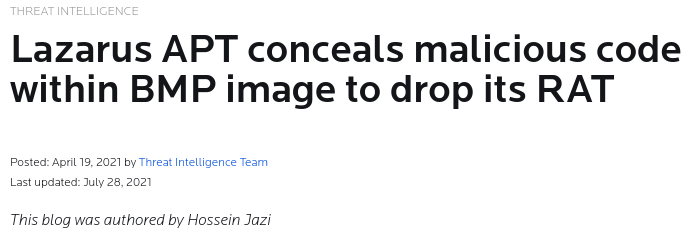
\includegraphics[scale=0.5]{images/rat_blog.png}
    \end{figure}
  \end{columns}
\end{frame}

\begin{frame}
  \frametitle{Lazarus APT BMP RAT Attack}
  \begin{columns}[T]
    \column{\textwidth}
    \begin{itemize}
      \item Uses a Microsoft Word document as a payload dropper
      \item Payload contains a PNG file with data appended
      \item Data is mistakenly extracted by a WIA function (\emph{WIA\_ConvertImage})
      \item Extracted data run using \emph{mshta} to drop second stage payload
      \item Second stage payload (\emph{AppStore.exe}) contains encrypted RAT, decrypted at runtime
    \end{itemize}
  \end{columns}
\end{frame}

% ------ Attack Recreation
\begin{frame}
  \frametitle{Malware Recreation}
  \begin{columns}[T]
    \column{\textwidth}
    \begin{itemize}
      \item We recreated only the executable concealment and the droppers
      \item Demo time!
    \end{itemize}
  \end{columns}
\end{frame}

% ------ E, D, C
\begin{frame}
  \frametitle{Evaluation, Discussion, Conclusions}
  \begin{columns}[T]
    \column{\textwidth}
    \begin{itemize}
      \item As is evident, the attack \emph{no longer works}
      \item Why? No clear answer, most likely a patch to the faulty \emph{WIA\_ConvertImage} function
      \item We ran into some difficulties with this function, possibly leading to inaccurate results
      \item We reached out for comment and clarification to Malwarebytes, but haven't received an answer
      \item Image concealment mechanism not known, unable to precisely recreate binwalk signature
    \end{itemize}
  \end{columns}
\end{frame}

\begin{frame}
  \frametitle{Evaluation, Discussion, Conclusions}
  \begin{itemize}
    \item Image concealment mechanism not known, unable to precisely recreate binwalk signature
    \item Failure to extract data possibly due to a patch
  \end{itemize}
  \begin{columns}[T]
    \column{0.5\textwidth}
    \begin{figure}[H]
      \centering
      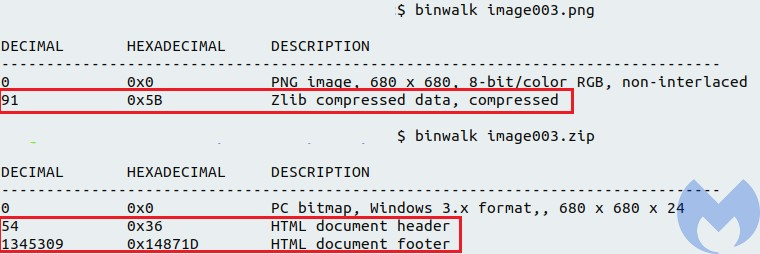
\includegraphics[scale=0.33]{images/malwarebytes_binwalk.jpg}
    \end{figure}
    \column{0.5\textwidth}
    \begin{figure}[H]
      \centering
      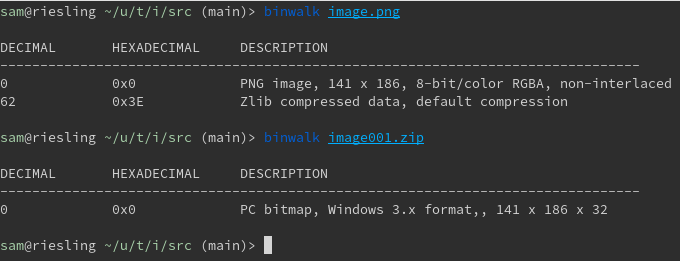
\includegraphics[scale=0.33]{images/my_binwalks.png}
    \end{figure}
  \end{columns}
\end{frame}

\begin{frame}
  \frametitle{Evaluation, Discussion, Conclusions}
  \begin{columns}[T]
    \column{\textwidth}
    \begin{itemize}
      \item Tested on Windows 10 (target OS for the attack) 
      \item Microsoft Word versions: 2019, 365
      \item We believe modern systems are \emph{no longer vulnerable} to this attack
      \item Vulnerability is likely to have been stealthily patched
    \end{itemize}
  \end{columns}
\end{frame}

\begin{frame}
  \frametitle{}
  Thank you for your attention!
\end{frame}
\end{document}
